% ---
% title: Recent Image Compression: Four Branches, 2025–2026
% date: 2026-10-13
% tag: Slides
% excerpt: A follow-up to From Samples to Bits. Since learned codecs caught up with VVC in 2020, research has split four ways. For each, two papers from 2025–2026, shown with their own pipeline figures: fewer bits at the same error (DCAE, HPCM), real-looking images from one diffusion step (StableCodec, OneDC), decoders small enough for a CPU (LotteryCodec, Good-Cheap-Fast), and images compressed for multimodal LLMs (transform-neck, CoTAM). JPEG AI (2025) shows where the four meet.
% ---
% About 18 minutes: opening 2 min, the four branches 3-3.5 min each, JPEG AI,
% summary and open problems 3 min. The comment above each frame gives a
% suggested time. Each paper's figure is its own, cut from its arXiv source;
% figures give width and height in pixels of the 960x540 slide, so a slide is
% fitted before its image loads.
\documentclass[aspectratio=169]{beamer}
\usetikzlibrary{arrows.meta,positioning,calc}
\definecolor{sig}{HTML}{1F5FAD}
\definecolor{hot}{HTML}{C0392B}
\definecolor{accent}{HTML}{C77C02}
\definecolor{soft}{HTML}{8C8C8C}
\definecolor{video}{HTML}{2E7D6B}

\title[Recent Image Compression]{Recent Image Compression}
\subtitle{Four branches of learned codecs, 2025--2026}
\author{Xu Chen}
\date{October 2026}

\begin{document}

% 0:15
\begin{frame}
  \titlepage
\end{frame}

% 1:00
\begin{frame}{Where we left off: one pipeline, one loss}
  \begin{center}
  \begin{tikzpicture}[nn, node distance=4mm, nndata/.append style={minimum width=8mm},
      mk/.style={circle, draw=#1, fill=#1!15, text=#1!70!black, inner sep=0pt, minimum size=5mm, font=\footnotesize\bfseries}]
    \node[nndata] (x) {$x$};
    \node[nnenc, right=of x] (ga) {$g_a$};
    \node[nnbox={nnactc}{9mm}, right=of ga] (q) {$Q$};
    \node[nnbox={nnfcc}{10mm}, right=of q] (ae) {AE};
    \node[right=of ae, font=\ttfamily\small] (bits) {bits};
    \node[nnbox={nnfcc}{10mm}, right=of bits] (ad) {AD};
    \node[nndec, right=of ad] (gs) {$g_s$};
    \node[nndata, right=of gs] (xh) {$\hat x$};
    \node[nnbox={nnnormc}{20mm}, above=6mm of bits] (p) {entropy model $p(\hat y)$};
    \draw[nnflow] (x) -- (ga);
    \draw[nnflow] (ga) -- (q);
    \draw[nnflow] (q) -- (ae);
    \draw[nnflow] (ae) -- (bits);
    \draw[nnflow] (bits) -- (ad);
    \draw[nnflow] (ad) -- (gs);
    \draw[nnflow] (gs) -- (xh);
    \draw[nnflow, dashed] (p.south -| ae) -- (ae);
    \draw[nnflow, dashed] (p.south -| ad) -- (ad);
    \coordinate (dl) at ($(ad.west |- gs.south)+(0,-0.2)$);
    \coordinate (dr) at ($(gs.east |- gs.south)+(0,-0.2)$);
    \draw[video, thick] (dl) -- ++(0,-0.2) -- ($(dr)+(0,-0.2)$) -- (dr);
    \node[mk=sig] at ($(ga.north)+(0,0.4)$) {1};
    \node[mk=sig] at ($(p.west)+(-0.4,0)$) {1};
    \node[mk=accent] at ($(gs.north)+(0,0.55)$) {2};
    \node[mk=video] at ($($(dl)!0.5!(dr)$)+(0,-0.55)$) {3};
    \node[mk=hot] at ($(xh.north)+(0,0.4)$) {4};
  \end{tikzpicture}
  \end{center}
  \[ \mathcal L \;=\; R + \lambda D \;=\; \mathbb E\big[-\log_2 p(\hat y)\big] + \lambda\,\mathbb E\big[\|x-\hat x\|^2\big] \]
  It matched VVC by 2020 \cite{balle2018,cheng2020}. Since then, four branches:
  \begin{center}
  \begin{tabular}{llll}
    \textcolor{sig}{\textbf{1 Rate}} & fewer bits, same error &
    \textcolor{video}{\textbf{3 Complexity}} & a decoder a phone can run \\
    \textcolor{accent}{\textbf{2 Perception}} & look real at 0.01 bpp &
    \textcolor{hot}{\textbf{4 Receiver}} & compress for a model \\
  \end{tabular}
  \end{center}
\end{frame}

% 0:45
\begin{frame}{Four branches, eight papers, one standard}
  \begin{center}
  \footnotesize
  \begin{tabular}{llll}
    \toprule
    Branch & Question & Key works & Venue \\
    \midrule
    \textcolor{sig}{1~Rate} & Fewer bits, same PSNR? & DCAE~\cite{lu2025dcae}, HPCM~\cite{li2025hpcm} & CVPR 2025, ICCV 2025 \\
    \textcolor{accent}{2~Perception} & Realism below 0.01 bpp? & StableCodec~\cite{zhang2025stablecodec}, OneDC~\cite{xue2025onedc} & ICCV 2025, NeurIPS 2025 \\
    \textcolor{video}{3~Complexity} & VVC at 4k MAC/pixel? & LotteryCodec~\cite{wu2025lottery}, C3/WD~\cite{balle2025gcf} & ICML 2025, CVPR 2025 \\
    \textcolor{hot}{4~Receiver} & Bits for an MLLM? & Transform-neck~\cite{kao2025neck}, CoTAM~\cite{liu2026cotam} & ICLR 2025, ICLR 2026 \\
    \midrule
    All four & What does a standard adopt? & JPEG AI~\cite{jpegai2025,esenlik2025} & ISO/IEC 2025 \\
    \bottomrule
  \end{tabular}
  \end{center}
  \medskip
  Yardstick: \textbf{BD-rate} against VTM (H.266/VVC, intra), the change in bits at equal quality; $-10\%$ means $10\%$ fewer bits.
\end{frame}

\section{Fewer bits at the same error}

% 1:00
\begin{frame}{Branch 1: the bits are only as good as the model}
  \begin{columns}[T]
    \begin{column}{0.56\textwidth}
      \begin{itemize}
        \item $\hat y_i$ costs $-\log_2 p(\hat y_i\mid\text{context})$ bits: better prediction, fewer bits.
        \item \textbf{Transform} $g_a$: pack the image into few numbers. Needs local texture \emph{and} long-range structure.
        \item \textbf{Entropy model} $p$: predict from what the decoder already has \cite{balle2018,he2022elic}.
        \item Both 2025 papers improve $p$.
      \end{itemize}
    \end{column}
    \begin{column}{0.44\textwidth}
      \begin{center}
      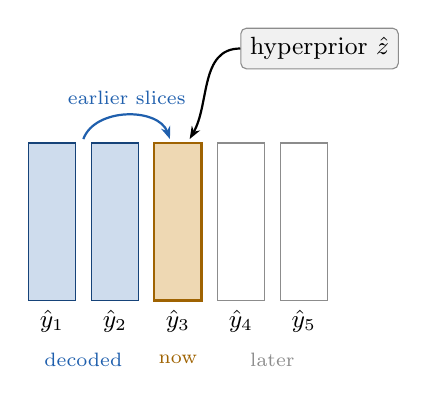
\begin{tikzpicture}[font=\small, >={Stealth[length=1.6mm]}]
        \foreach \i in {0,1}
          \filldraw[draw=sig!70!black, fill=sig!22] (0.8*\i,0) rectangle ++(0.6,2);
        \filldraw[draw=accent!80!black, fill=accent!30, thick] (1.6,0) rectangle ++(0.6,2);
        \foreach \i in {3,4}
          \draw[soft] (0.8*\i,0) rectangle ++(0.6,2);
        \foreach \i in {1,...,5}
          \node[below] at ({0.8*\i-0.5},0) {$\hat y_{\i}$};
        \node[sig, font=\scriptsize] at (0.7,-0.75) {decoded};
        \node[accent!80!black, font=\scriptsize] at (1.9,-0.75) {now};
        \node[soft, font=\scriptsize] at (3.1,-0.75) {later};
        \node[draw=soft, fill=soft!12, rounded corners=2pt] (z) at (3.7,3.2) {hyperprior $\hat z$};
        \draw[->, thick] (z.west) to[out=180, in=60] (2.05,2.05);
        \draw[->, thick, sig] (0.7,2.05) to[out=70, in=110] node[above, font=\scriptsize] {earlier slices} (1.8,2.05);
      \end{tikzpicture}
      \end{center}
      {\small Slices of $\hat y$ are decoded in order.}
    \end{column}
  \end{columns}
\end{frame}

% 1:10
\begin{frame}{DCAE (CVPR 2025): a dictionary as prior}
  \begin{center}
  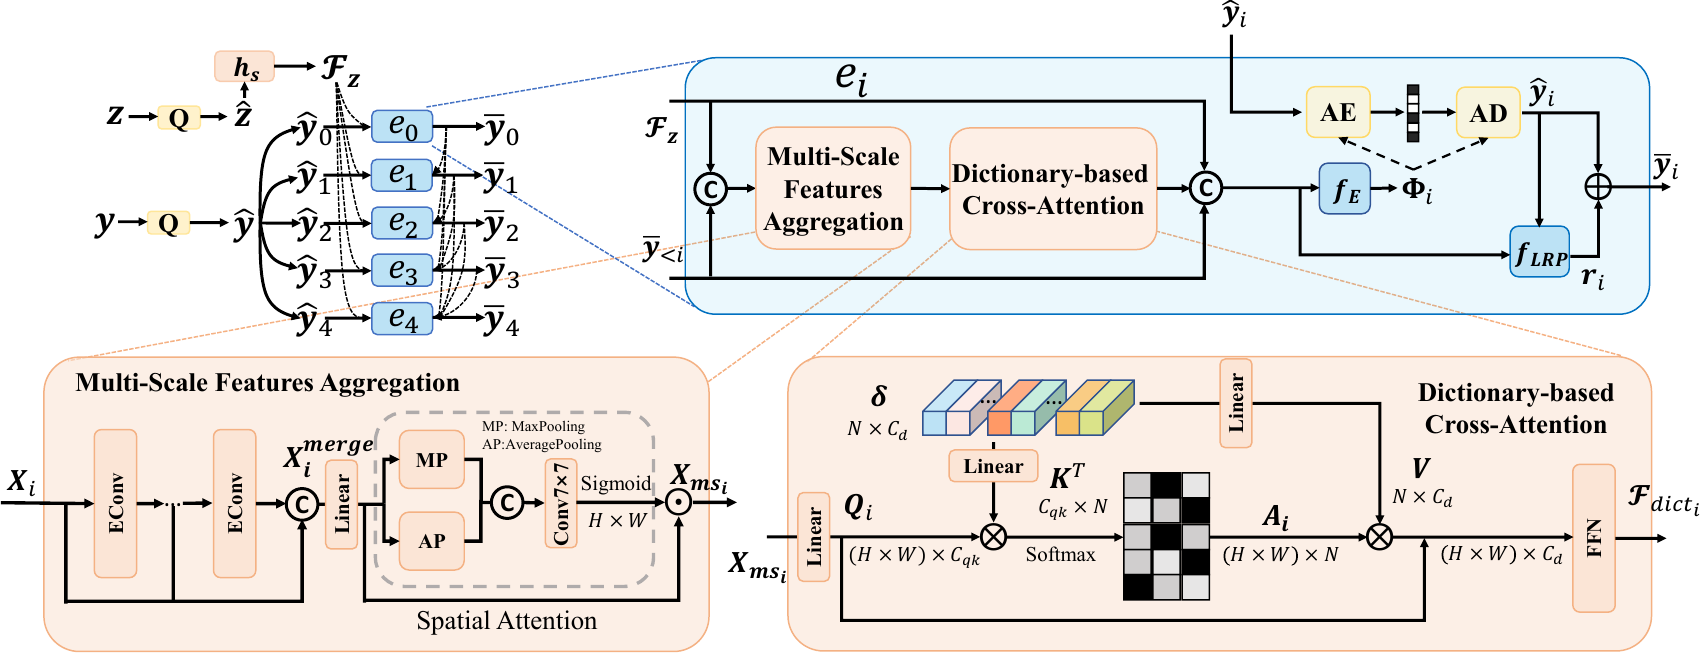
\includegraphics[width=850px,height=327px]{notes/assets/recent-image-compression/dcae.png}

  {\scriptsize Figure from \cite{lu2025dcae}.}
  \end{center}
  \begin{itemize}
    \item \textbf{Problem.} Entropy models look only inside the image; structures recur across images.
    \item \textbf{Method.} A learned dictionary ($128\times640$, never sent), read by cross-attention.
    \item \textbf{Result.} $-17.0/{-21.1}/{-19.7}\%$ vs.\ VTM-12.1 (Kodak, Tecnick, CLIC); 193 ms, MLIC++ 772 ms.
  \end{itemize}
\end{frame}

% 1:10
\begin{frame}{HPCM (ICCV 2025): context from coarse to fine}
  \begin{center}
  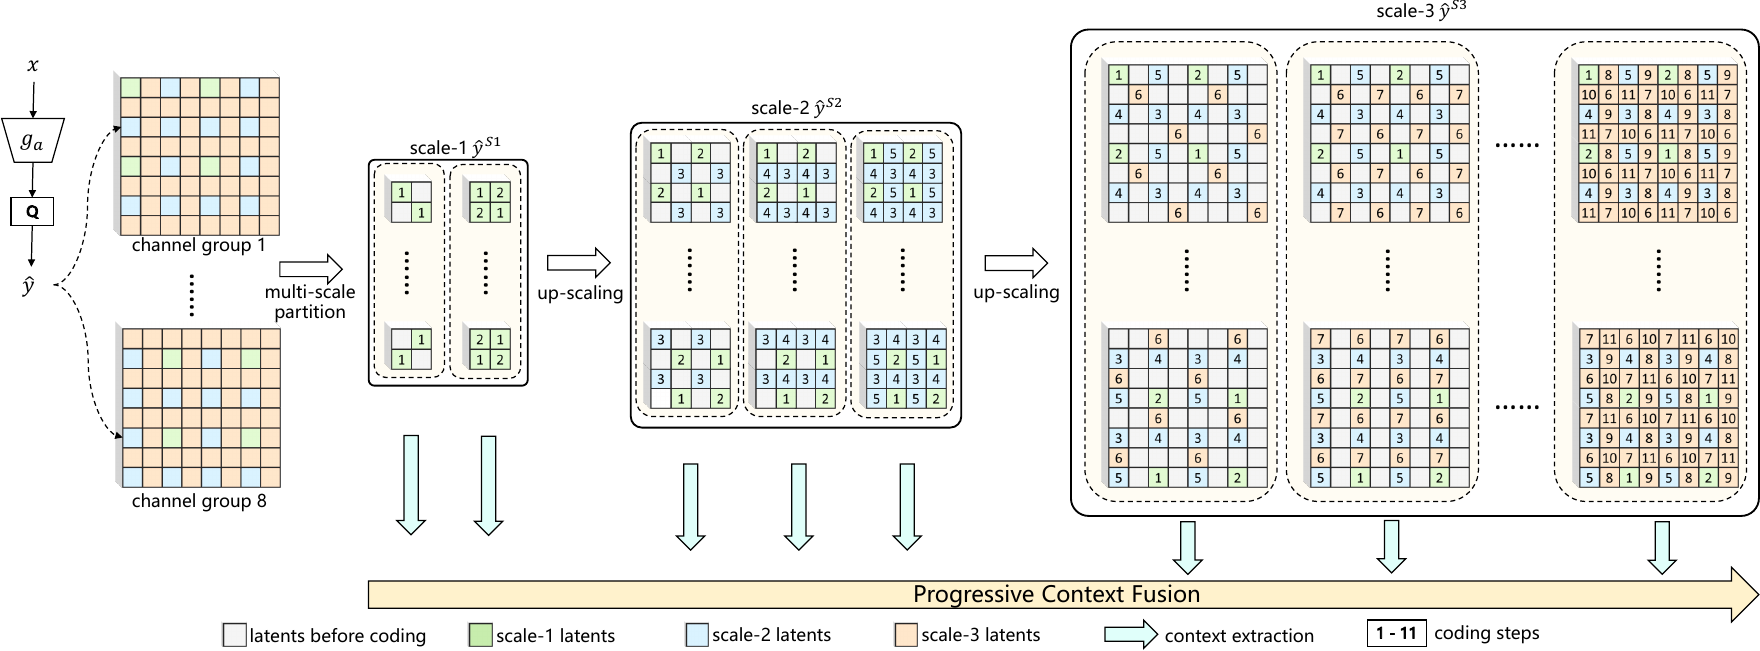
\includegraphics[width=850px,height=314px]{notes/assets/recent-image-compression/hpcm.png}

  {\scriptsize Figure from \cite{li2025hpcm}.}
  \end{center}
  \begin{itemize}
    \item \textbf{Problem.} Long-range context is costly; each step forgets what earlier steps found.
    \item \textbf{Method.} Code $\hat y$ at three scales, smallest first ($2+3+6$ steps); cross-attention carries context.
    \item \textbf{Result.} $-19.2/{-22.2}/{-18.4}\%$ vs.\ VTM-22.0 (Kodak, Tecnick, CLIC); 90 ms, MLIC++ 226 ms.
  \end{itemize}
\end{frame}

\section{Real-looking images from a few hundred bytes}

% 1:00
\begin{frame}{Branch 2: exact or realistic, not both}
  \begin{columns}[T]
    \begin{column}{0.52\textwidth}
      \begin{itemize}
        \item At low rates the MSE-optimal decoder outputs the \textbf{average} $\mathbb E[x\mid\text{bits}]$: blurry.
        \item At a fixed rate, more realism costs more distortion \cite{blau2018,blau2019}.
        \item So: send \textbf{structure}, let diffusion \textbf{invent texture}. In 2025, in \emph{one} step.
      \end{itemize}
    \end{column}
    \begin{column}{0.48\textwidth}
      \begin{center}
      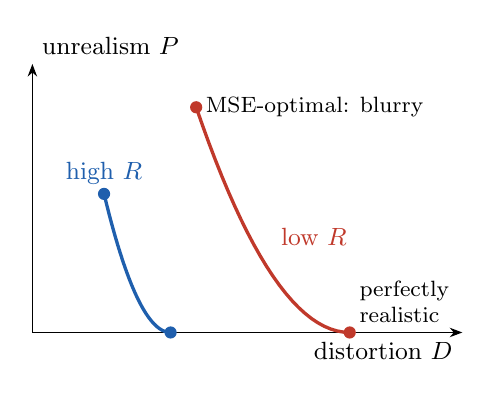
\begin{tikzpicture}[x=1.3cm, y=1.1cm, font=\small, >={Stealth[length=1.6mm]}]
        \draw[->] (0,0) -- (4.2,0) node[below left] {distortion $D$};
        \draw[->] (0,0) -- (0,3.1) node[above right] {unrealism $P$};
        \draw[sig, very thick, domain=0.7:1.35] plot (\x, {3.787*(1.35-\x)^2});
        \draw[hot, very thick, domain=1.6:3.1] plot (\x, {1.156*(3.1-\x)^2});
        \fill[sig] (0.7,1.6) circle (2.2pt) node[above, font=\small] {high $R$};
        \fill[sig] (1.35,0) circle (2.2pt);
        \node[hot] at (2.75,1.1) {low $R$};
        \fill[hot] (1.6,2.6) circle (2.2pt) node[right, black, font=\footnotesize] {MSE-optimal: blurry};
        \fill[hot] (3.1,0) circle (2.2pt) node[above right, black, font=\footnotesize, align=left] {perfectly\\realistic};
      \end{tikzpicture}
      \end{center}
      {\small Schematic, after \cite{blau2019}: perfect realism at most doubles the MSE.}
    \end{column}
  \end{columns}
  \medskip
  \alert{Generated, not transmitted}: it looks right, but may not be what the camera saw.
\end{frame}

% 1:10
\begin{frame}{StableCodec (ICCV 2025): diffusion in one step}
  \begin{center}
  \includegraphics[width=850px,height=227px]{notes/assets/recent-image-compression/stablecodec.webp}

  {\scriptsize Figure and table from \cite{zhang2025stablecodec}.}
  \end{center}
  \begin{columns}[T]
    \begin{column}{0.55\textwidth}
      \begin{itemize}
        \item \textbf{Problem.} 20--50 steps; drift from the pixels.
        \item \textbf{Method.} Send a \emph{noisy latent} $l_T$; one SD-Turbo step \cite{sauer2024} cleans it; a side branch keeps structure.
        \item \textbf{Result.} Best FID, DISTS to 0.005 bpp.
      \end{itemize}
    \end{column}
    \begin{column}{0.45\textwidth}
      \begin{center}
      \footnotesize
      \begin{tabular}{lrr}
        \toprule
        Kodak,~RTX~3090 & steps & decoding \\
        \midrule
        DiffEIC~\cite{li2024diffeic} & 50 & 7.42 s \\
        PerCo~\cite{careil2024perco} & 20 & 3.74 s \\
        \textbf{StableCodec} & \textbf{1} & \textbf{0.33 s} \\
        MS-ILLM (GAN) \cite{muckley2023} & -- & 0.32 s \\
        \bottomrule
      \end{tabular}
      \end{center}
    \end{column}
  \end{columns}
\end{frame}

% 1:10
\begin{frame}{OneDC (NeurIPS 2025): hyperprior as prompt}
  \begin{center}
  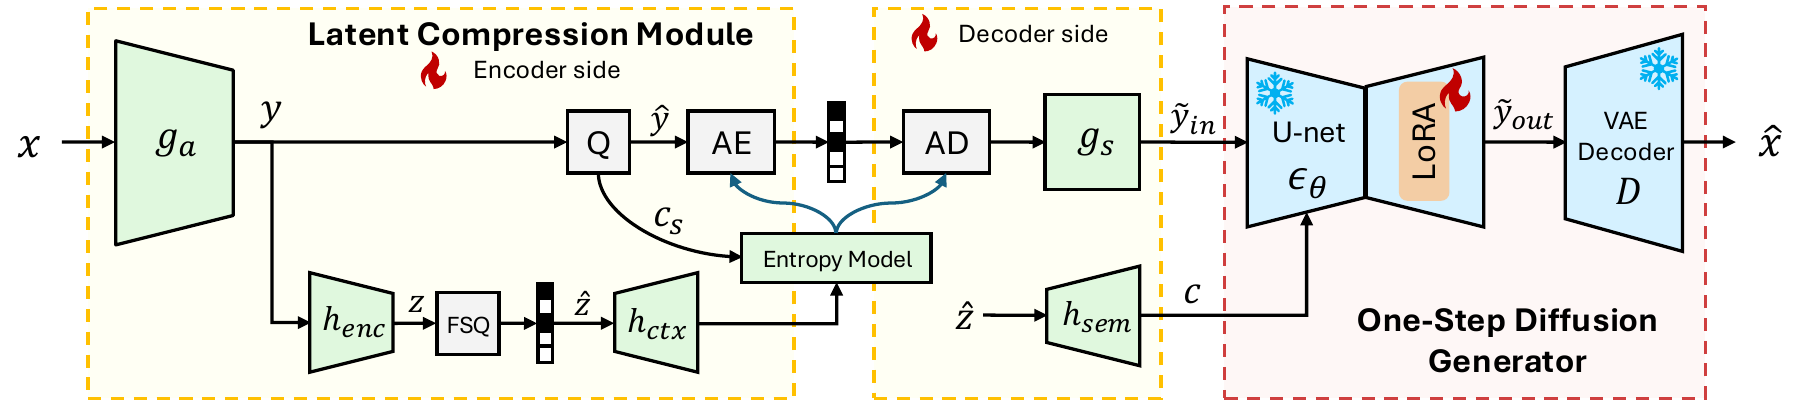
\includegraphics[width=850px,height=193px]{notes/assets/recent-image-compression/onedc.png}

  {\scriptsize Figure from \cite{xue2025onedc}.}
  \end{center}
  \begin{itemize}
    \item \textbf{Problem.} One step needs strong guidance; text cannot say \emph{where} things are.
    \item \textbf{Method.} Hyperprior tokens $\hat z$ (0.0034 bpp) replace the text; MaskGIT \cite{chang2022maskgit} teaches them.
    \item \textbf{Result.} $39.6\%$ fewer bits than PerCo at equal FID (MS-COCO); 0.34 s vs.\ 8.8 s to decode.
  \end{itemize}
\end{frame}

\section{Decoders small enough for a CPU}

% 1:00
\begin{frame}{Branch 3: fit a tiny decoder to each image}
  \begin{center}
  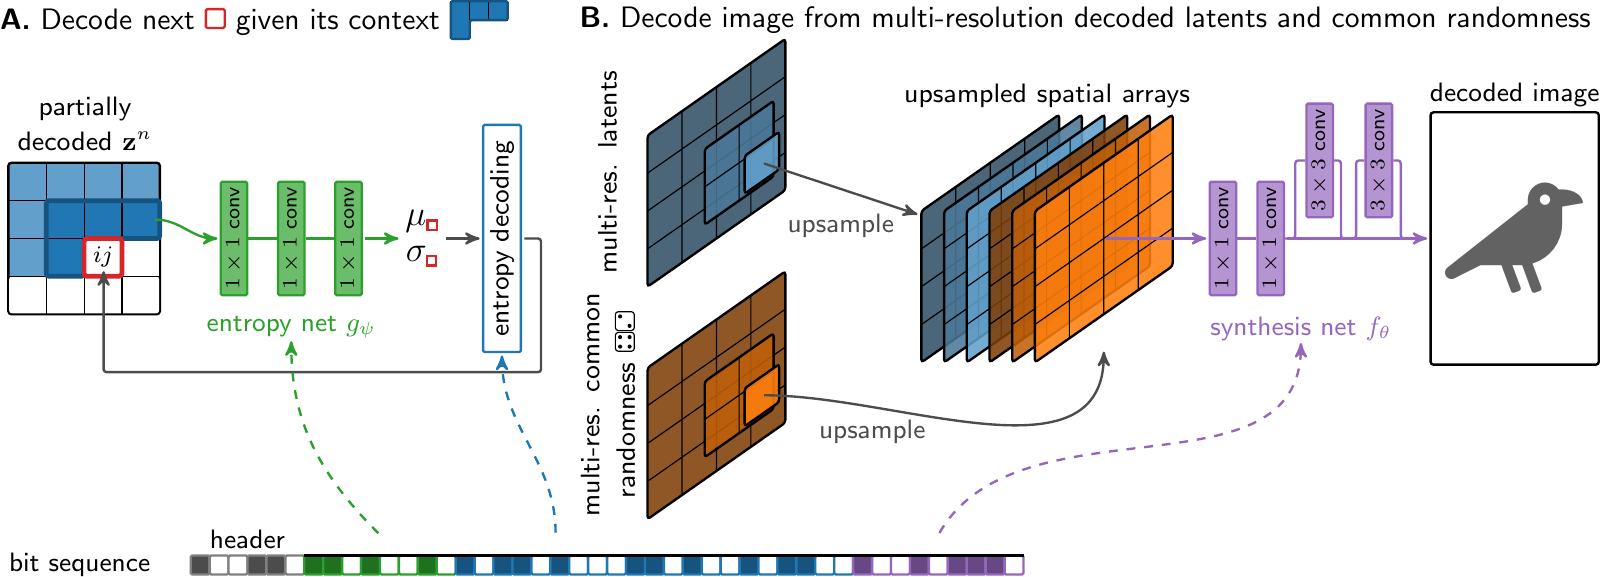
\includegraphics[width=800px,height=289px]{notes/assets/recent-image-compression/c3.png}

  {\scriptsize Decoding in Cool-Chic and C3; figure from \cite{balle2025gcf}.}
  \end{center}
  \begin{itemize}
    \item \textbf{Problem.} One decoder for every image is big: JPEG AI's take 13--215 kMAC/pixel \cite{esenlik2025}.
    \item \textbf{Idea: overfit} a tiny model to \emph{this} image, and send it. Cool-Chic \cite{ladune2023coolchic}, C3 \cite{kim2024c3}: $\sim$3k MAC/pixel.
    \item \alert{The cost moves to the encoder}: each image is a training run.
  \end{itemize}
\end{frame}

% 1:10
\begin{frame}{LotteryCodec (ICML 2025): a mask, not weights}
  \begin{center}
  \includegraphics[width=640px,height=316px]{notes/assets/recent-image-compression/lottery.webp}

  {\scriptsize Figure from \cite{wu2025lottery}.}
  \end{center}
  \begin{itemize}
    \item \textbf{Problem.} An overfitted codec sends its decoder's weights; at low rates they eat the bits.
    \item \textbf{Method.} A random net from a shared seed hides a good decoder: send the mask that picks it.
    \item \textbf{Result.} Past VTM-19.1 (up to $-9.8\%$, CLIC) at $\sim$4k MAC/pixel; the mask ratio trades the two.
  \end{itemize}
\end{frame}

% 1:10
\begin{frame}{Good, Cheap, and Fast (CVPR 2025)}
  \begin{center}
  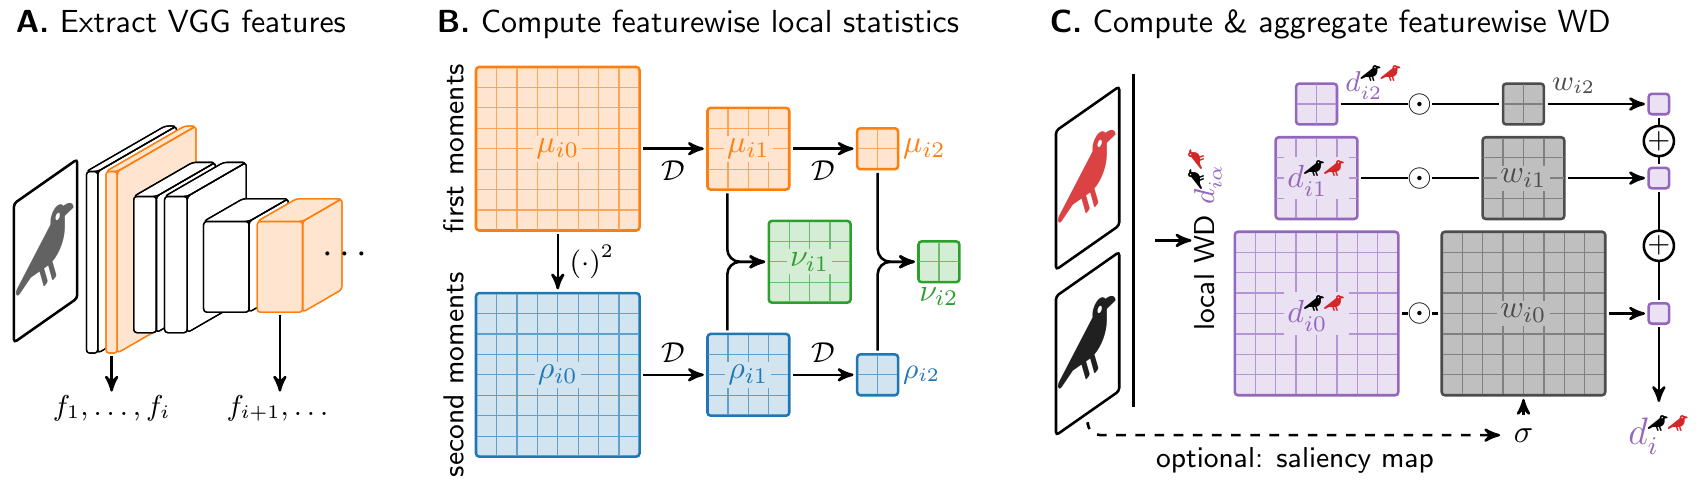
\includegraphics[width=850px,height=244px]{notes/assets/recent-image-compression/wd.png}

  {\scriptsize Wasserstein Distortion; figure from \cite{balle2025gcf}.}
  \end{center}
  \begin{itemize}
    \item \textbf{Problem.} Realistic codecs take $10^5$--$10^6$ MAC/pixel; cheap overfitted ones look flat.
    \item \textbf{Method.} Train C3 for \emph{Wasserstein Distortion}: match local VGG statistics, not pixels.
    \item \textbf{Result.} Human study, 0.15 bpp: on par with HiFiC \cite{mentzer2020hific} at 3.1k vs.\ 609k MAC/pixel.
  \end{itemize}
\end{frame}

\section{Compressing for a model, not an eye}

% 0:50
\begin{frame}{Branch 4: when the receiver is an MLLM}
  \begin{center}
  \includegraphics[width=700px,height=328px]{notes/assets/recent-image-compression/neck-teaser.webp}

  {\scriptsize Figure from \cite{kao2025neck}.}
  \end{center}
  \begin{itemize}
    \item \textbf{Problem.} A codec for people wastes bits (a); training through the MLLM costs too much (b, c).
    \item \textbf{2025--2026}: adapt to the MLLM's \emph{vision encoder}, never the LLM.
  \end{itemize}
\end{frame}

% 1:10
\begin{frame}{Transform-neck (ICLR 2025): skip the pixels}
  \begin{center}
  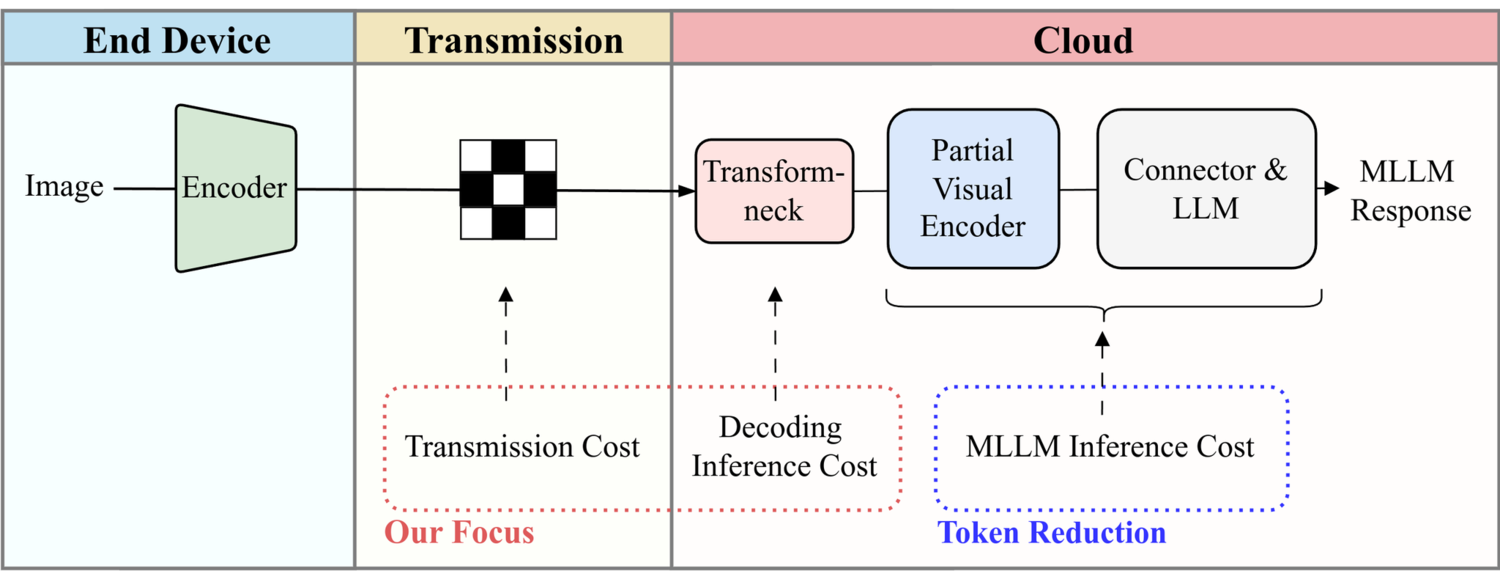
\includegraphics[width=760px,height=289px]{notes/assets/recent-image-compression/neck.png}

  {\scriptsize Figure from \cite{kao2025neck}.}
  \end{center}
  \begin{itemize}
    \item \textbf{Problem.} Decoded images hurt MLLMs at low rates; the LLM is too big to train through.
    \item \textbf{Method.} A 13M-parameter neck maps $\hat y$ into CLIP \cite{radford2021clip}, trained on CLIP's features alone.
    \item \textbf{Result.} 60--80\% fewer bits at equal accuracy; 53 instead of 1018 kMAC/pixel after the bits.
  \end{itemize}
\end{frame}

% 1:10
\begin{frame}{CoTAM (ICLR 2026): bits where CLIP looks}
  \begin{center}
  \includegraphics[width=850px,height=203px]{notes/assets/recent-image-compression/cotam.webp}

  {\scriptsize Training (left) and inference (right); figure from \cite{liu2026cotam}.}
  \end{center}
  \begin{itemize}
    \item \textbf{Problem.} Compression first breaks the features that join detail to context.
    \item \textbf{Method.} CLIP's first three layers steer the bits; a one-block adapter feeds the MLLM.
    \item \textbf{Result.} LLaVA-1.5, six tasks: $36\%$ fewer bits than ELIC at equal score; $31\%$ on DCAE.
  \end{itemize}
\end{frame}

\section{Where the branches meet}

% 1:00
\begin{frame}{JPEG AI (2025): where the branches meet}
  \begin{columns}[T]
    \begin{column}{0.46\textwidth}
      \begin{center}
      \includegraphics[width=380px,height=371px]{notes/assets/recent-image-compression/jpegai.webp}

      {\scriptsize The decoder; figure from \cite{esenlik2025}.}
      \end{center}
    \end{column}
    \begin{column}{0.54\textwidth}
      \begin{itemize}
        \item First learned image standard: ISO/IEC 6048-1, 2025 \cite{jpegai2025}.
        \item \textcolor{sig}{\textbf{Rate}}: $-14\%$ to $-27\%$ vs.\ VVC intra.
        \item \textcolor{video}{\textbf{Complexity}}: one bitstream, three decoders: 13, 28, 215 kMAC/pixel.
        \item \textbf{Bit-exact}: integer entropy decoding on every device.
        \item \textcolor{hot}{\textbf{Receiver}}: machines in scope; v1 is for viewing.
      \end{itemize}
    \end{column}
  \end{columns}
\end{frame}

% 1:00
\begin{frame}{Four branches in one table}
  \begin{center}
  \footnotesize
  \begin{tabular}{llll}
    \toprule
    Branch & Problem & Method & What it reached \\
    \midrule
    \textcolor{sig}{1~Rate} & fewer bits, same PSNR & better entropy models & $-17\%$ to $-19\%$ vs.\ VTM (Kodak) \\
    \textcolor{accent}{2~Perception} & realism below 0.01 bpp & one guided diffusion step & 0.3 s instead of 4--12 s \\
    \textcolor{video}{3~Complexity} & decode on a CPU & overfit a tiny decoder & past VTM, or HiFiC-like, at $\le$4k MAC/px \\
    \textcolor{hot}{4~Receiver} & images read by MLLMs & adapt to the vision encoder & 30--80\% fewer bits, same accuracy \\
    \bottomrule
  \end{tabular}
  \end{center}
  \bigskip
  Each branch \alert{moves a cost}: more decoder compute (1), invented detail (2), slow encoding (3), ties to one vision encoder (4).
\end{frame}

% 0:50
\begin{frame}{Open problems}
  \begin{itemize}
    \item \textbf{Trusting generated detail}: text and faces can be invented; metrics cannot tell sent from made up.
    \item \textbf{Fast encoding} for overfitted codecs: each image is still a training run.
    \item \textbf{Decoding everywhere}: bit-exact on every device, and parallel.
    \item \textbf{One bitstream, many receivers}: people and MLLMs from the same bits.
    \item \textbf{Trend}: codecs built on pretrained models (diffusion U-Nets, tokenizers, CLIP).
  \end{itemize}
\end{frame}

% 0:00
\begin{frame}[t]
  \tiny
  \begin{thebibliography}{99}
    \bibitem{balle2018} J. Ball\'e, D. Minnen, S. Singh, S. J. Hwang, N. Johnston. Variational image compression with a scale hyperprior. \emph{ICLR}, 2018.
    \bibitem{cheng2020} Z. Cheng, H. Sun, M. Takeuchi, J. Katto. Learned image compression with discretized Gaussian mixture likelihoods and attention modules. \emph{CVPR}, 2020.
    \bibitem{lu2025dcae} J. Lu, L. Zhang, X. Zhou, M. Li, W. Li, S. Gu. Learned image compression with dictionary-based entropy model. \emph{CVPR}, 2025.
    \bibitem{li2025hpcm} Y. Li, H. Zhang, L. Li, D. Liu. Learned image compression with hierarchical progressive context modeling. \emph{ICCV}, 2025.
    \bibitem{zhang2025stablecodec} T. Zhang, X. Luo, L. Li, D. Liu. StableCodec: taming one-step diffusion for extreme image compression. \emph{ICCV}, 2025.
    \bibitem{xue2025onedc} N. Xue, Z. Jia, J. Li, B. Li, Y. Zhang, Y. Lu. One-step diffusion-based image compression with semantic distillation. \emph{NeurIPS}, 2025.
    \bibitem{wu2025lottery} H. Wu, G. Chen, P. L. Dragotti, D. G\"und\"uz. LotteryCodec: searching the implicit representation in a random network for low-complexity image compression. \emph{ICML}, 2025.
    \bibitem{balle2025gcf} J. Ball\'e, L. Versari, E. Dupont, H. Kim, M. Bauer. Good, cheap, and fast: overfitted image compression with Wasserstein distortion. \emph{CVPR}, 2025.
    \bibitem{kao2025neck} C.-H. Kao, C. Chien, Y.-J. Tseng, Y.-H. Chen, A. Gnutti, S.-Y. Lo, W.-H. Peng, R. Leonardi. Bridging compressed image latents and multimodal large language models. \emph{ICLR}, 2025.
    \bibitem{liu2026cotam} J. Liu, Z. Jia, J. Li, B. Li, X. Jin, W. Zeng, Y. Lu. When MLLMs meet compression distortion: a coding paradigm tailored to MLLMs. \emph{ICLR}, 2026.
    \bibitem{jpegai2025} ISO/IEC 6048-1:2025. JPEG AI learning-based image coding system, Part 1: Core coding system.
    \bibitem{esenlik2025} S. Esenlik et al. An overview of the JPEG AI learning-based image coding standard. \emph{IEEE TCSVT}, 2025.
  \end{thebibliography}
\end{frame}

% 0:00
\begin{frame}[t]
  \tiny
  \begin{thebibliography}{99}
    \bibitem{he2022elic} D. He et al. ELIC: efficient learned image compression with unevenly grouped space-channel contextual adaptive coding. \emph{CVPR}, 2022.
    \bibitem{jiang2023mlic} W. Jiang, J. Yang, Y. Zhai, F. Gao, R. Wang. MLIC++: linear complexity multi-reference entropy modeling for learned image compression. \emph{ACM TOMM}, 2025.
    \bibitem{blau2018} Y. Blau, T. Michaeli. The perception--distortion tradeoff. \emph{CVPR}, 2018.
    \bibitem{blau2019} Y. Blau, T. Michaeli. Rethinking lossy compression: the rate-distortion-perception tradeoff. \emph{ICML}, 2019.
    \bibitem{sauer2024} A. Sauer, D. Lorenz, A. Blattmann, R. Rombach. Adversarial diffusion distillation. \emph{ECCV}, 2024.
    \bibitem{li2024diffeic} Z. Li, Y. Zhou, H. Wei, C. Ge, J. Jiang. Toward extreme image compression with latent feature guidance and diffusion prior. \emph{IEEE TCSVT}, 2025.
    \bibitem{careil2024perco} M. Careil, M. J. Muckley, J. Verbeek, S. Lathuili\`ere. Towards image compression with perfect realism at ultra-low bitrates. \emph{ICLR}, 2024.
    \bibitem{muckley2023} M. J. Muckley, A. El-Nouby, K. Ullrich, H. J\'egou, J. Verbeek. Improving statistical fidelity for neural image compression with implicit local likelihood models. \emph{ICML}, 2023.
    \bibitem{chang2022maskgit} H. Chang, H. Zhang, L. Jiang, C. Liu, W. T. Freeman. MaskGIT: masked generative image transformer. \emph{CVPR}, 2022.
    \bibitem{ladune2023coolchic} T. Ladune, P. Philippe, F. Henry, G. Clare, T. Leguay. COOL-CHIC: coordinate-based low complexity hierarchical image codec. \emph{ICCV}, 2023.
    \bibitem{kim2024c3} H. Kim, M. Bauer, L. Theis, J. R. Schwarz, E. Dupont. C3: high-performance and low-complexity neural compression from a single image or video. \emph{CVPR}, 2024.
    \bibitem{mentzer2020hific} F. Mentzer, G. Toderici, M. Tschannen, E. Agustsson. High-fidelity generative image compression. \emph{NeurIPS}, 2020.
    \bibitem{radford2021clip} A. Radford et al. Learning transferable visual models from natural language supervision. \emph{ICML}, 2021.
  \end{thebibliography}
\end{frame}

% 0:10
\begin{frame}[plain]
  \begin{center}
    {\Huge Thank you}

    \bigskip
    {\Large Questions?}
  \end{center}
\end{frame}

\end{document}
